\chapter{Results}
\label{sec:Results}

In this section the results of the cross-section calculations are presented. The results of the integral and differential cross-sections (as defined in Sec.~\ref{sec:ZeeCrossSec}) are shown together with uncertainties and theoretical predictions. There are two main types of the uncertainties: statistical and systematical, and whereas the statistical uncertainties are trivial to calculate, and depend only on the amount of the data in any given bin, the sources for the systematical uncertainties are much more numerous. The sources for the different systematical uncertainties are described throughout this thesis, but for the convinience the complete list of them that contributed to the final result is presented in Tab.~\ref{tab:Zee_unc_list}.

\begin{table}
\centering
\begin{tabular}{lcc}
\hline
   & peak mass & high mass  \\
\hline
Trigger efficiency                       & 0.050 & 0.048 \\
Recon. efficiency                        & 0.128 & 0.120 \\
Id. efficiency                           & 0.121 & 0.126 \\
Id.Fwd efficiency                        & 1.514 & 1.506 \\
Isol. efficiency                         & 0.039 & 0.052 \\
Electron resolution                      & 0.011 & 0.915 \\
Electron scale                           & 0.115 & 0.474 \\
Fwd Electron scale                       & 0.179 & 2.166 \\
pT Rew.                                  & 0.043 & 0.153 \\
Matrix element                           & 1.120 & 0.301 \\
PS and hadronization                     & 1.250 & 1.762 \\
Theory: PDF                              & 0.059 & 0.119 \\
EW Bkg                                   & 0.139 & 3.428 \\
QCD Bkg                                  & 0.052 & 3.802 \\
\hline
Tot. Syst. Uncertainty                   & 2.288 & 6.216 \\
\hline
\end{tabular}
\caption{The list of the systematic uncertainties in percent.}
\label{tab:Zee_unc_list}
\end{table}

As the work that was done as part of this thesis contributed to the W,Z inclusive paper~\cite{lib:wz2011} all the results were taken from there, including the theory comparison that was done for the combined \Zll\ results, and were thus, strictly speaking, outside of the scope of this thesis.

The double-differential were done in the rapidity and mass binning with three mass bins. The \Zee\ central-forward analysis contributed only to two of them: the peak mass ($66 < M_{ee} < 116$~GeV) and the high mass ($116 < M_{ee} < 150$~GeV) windows. Fig.~\ref{fig:res_zee_fid} shows the double-diffirential cross-section with statistical and systematical uncertainties, and Fig.~\ref{fig:res_zee_fid_norm} shows the comparison with the \Powheg\ and \Mcatnlo\ simulations.

\begin{figure}
\center{
  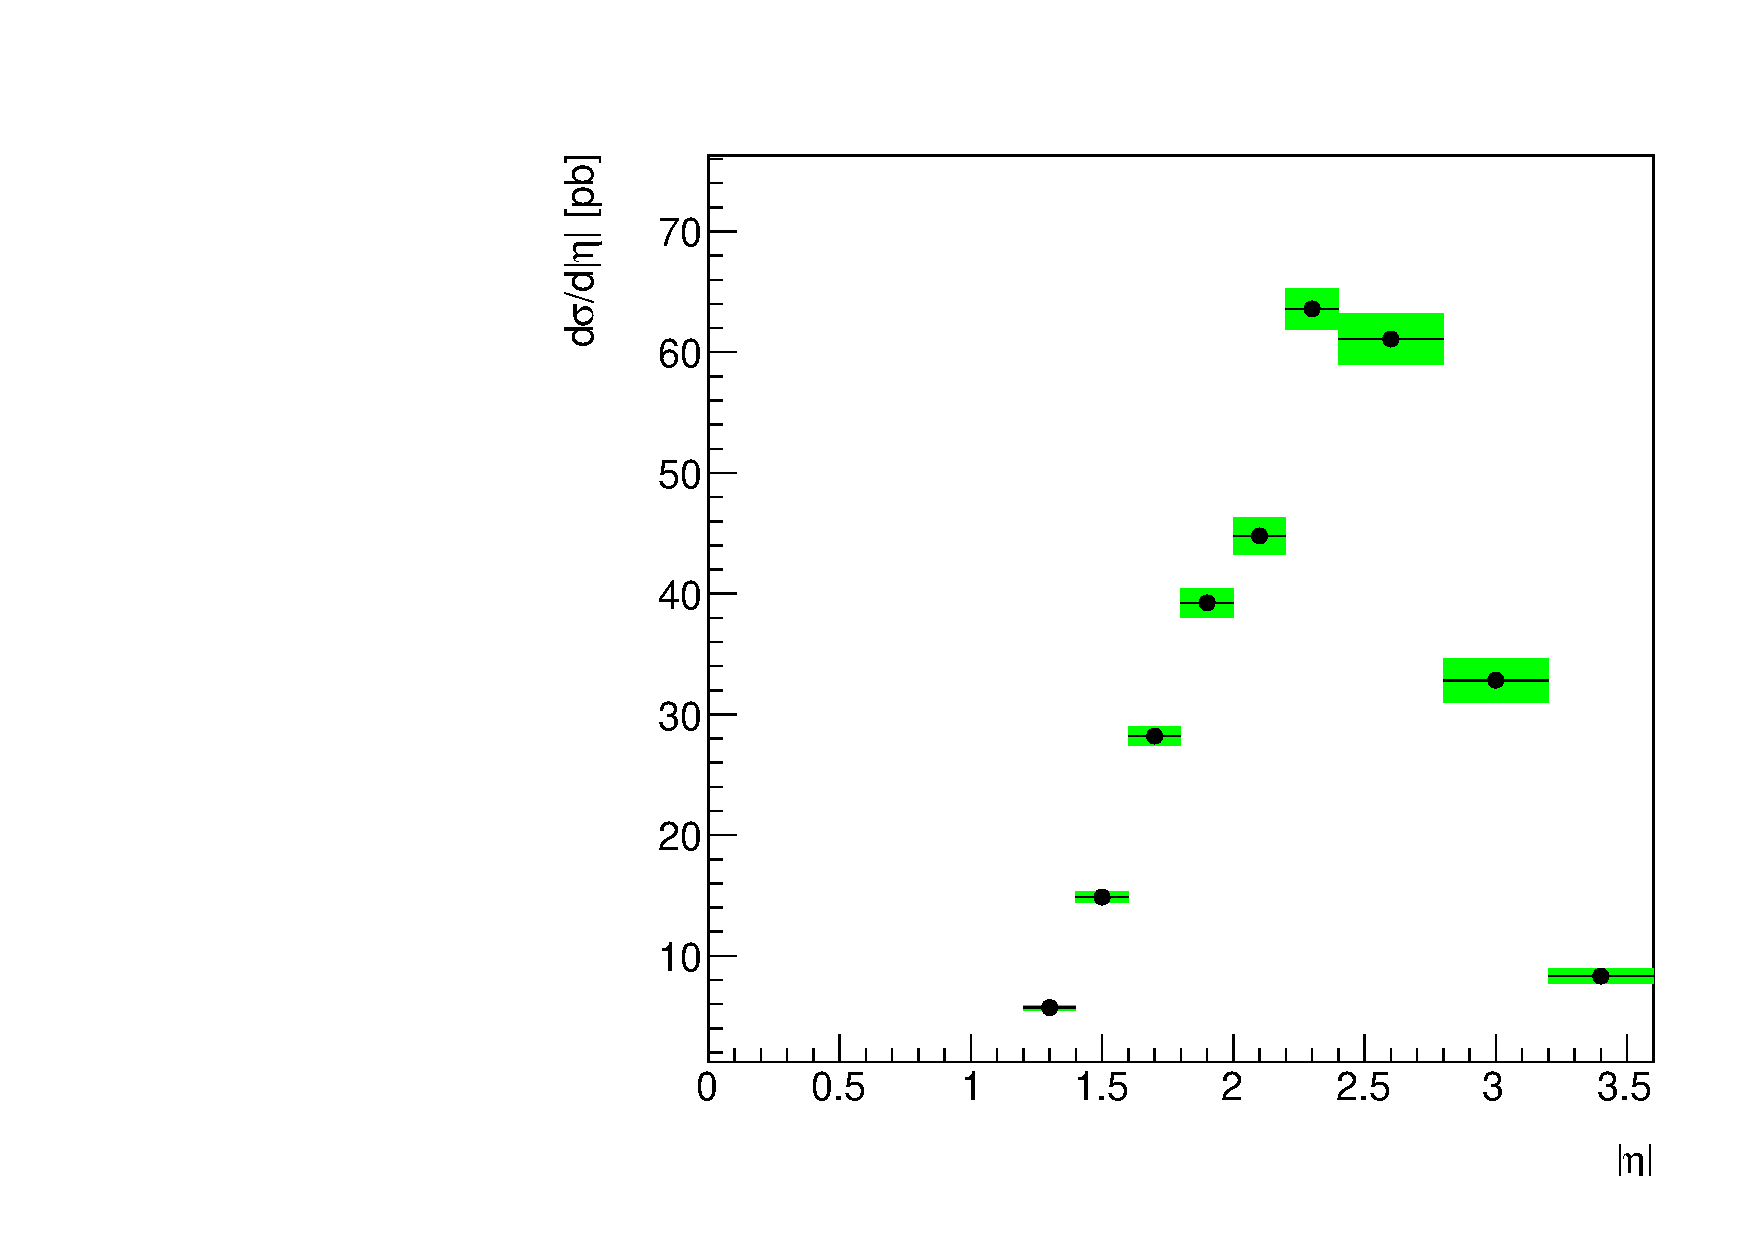
\includegraphics[width=0.45\textwidth]{figures/ZeeCF_Mass_66_116_FiduCS_band.pdf}
  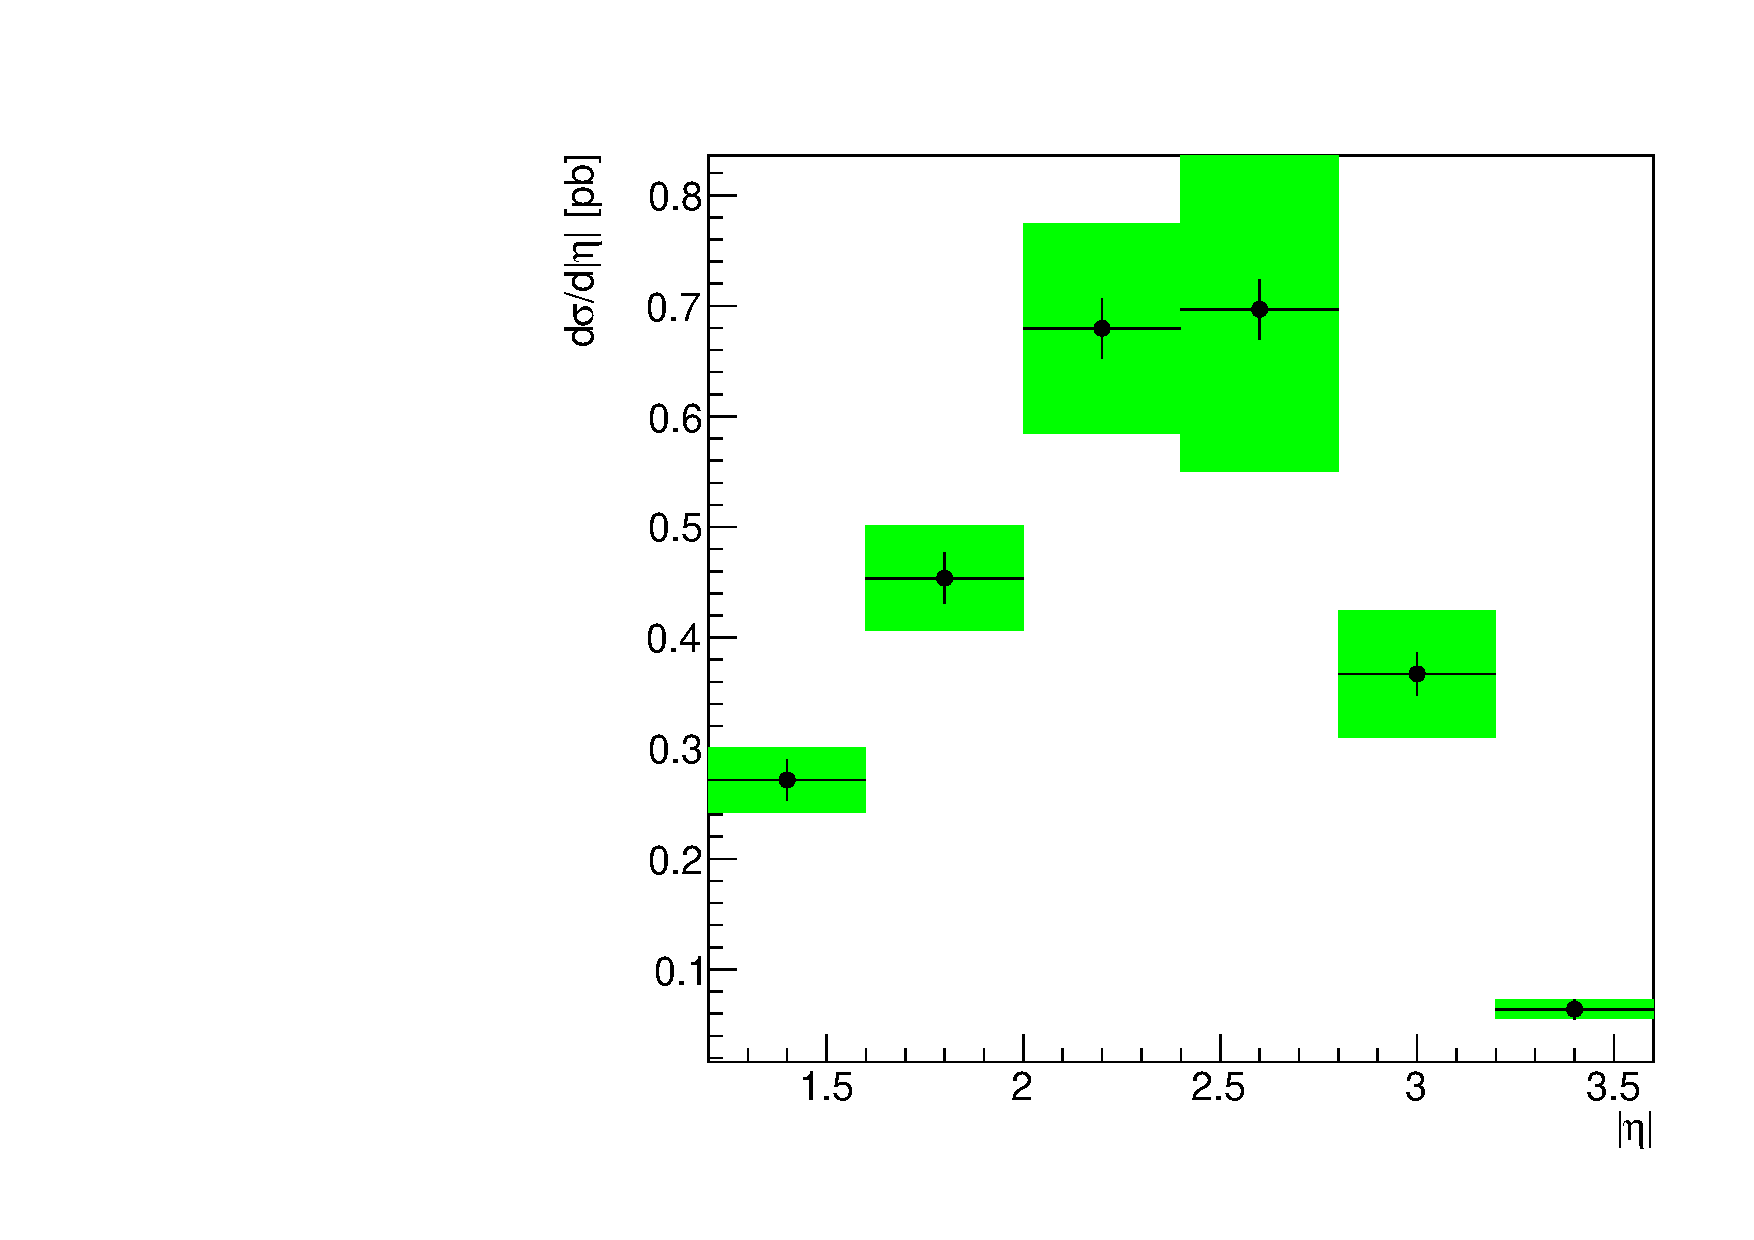
\includegraphics[width=0.45\textwidth]{figures/ZeeCF_Mass_116_150_FiduCS_band.pdf}
  \caption{\Zee\ CF fiducial diffirential cross-section, as a function of absolute boson rapidity for peak mass (left) and high mass (right) regions together with statistical and systematic uncertainties.}
\label{fig:res_zee_fid}}
\end{figure}

\begin{figure}
\center{
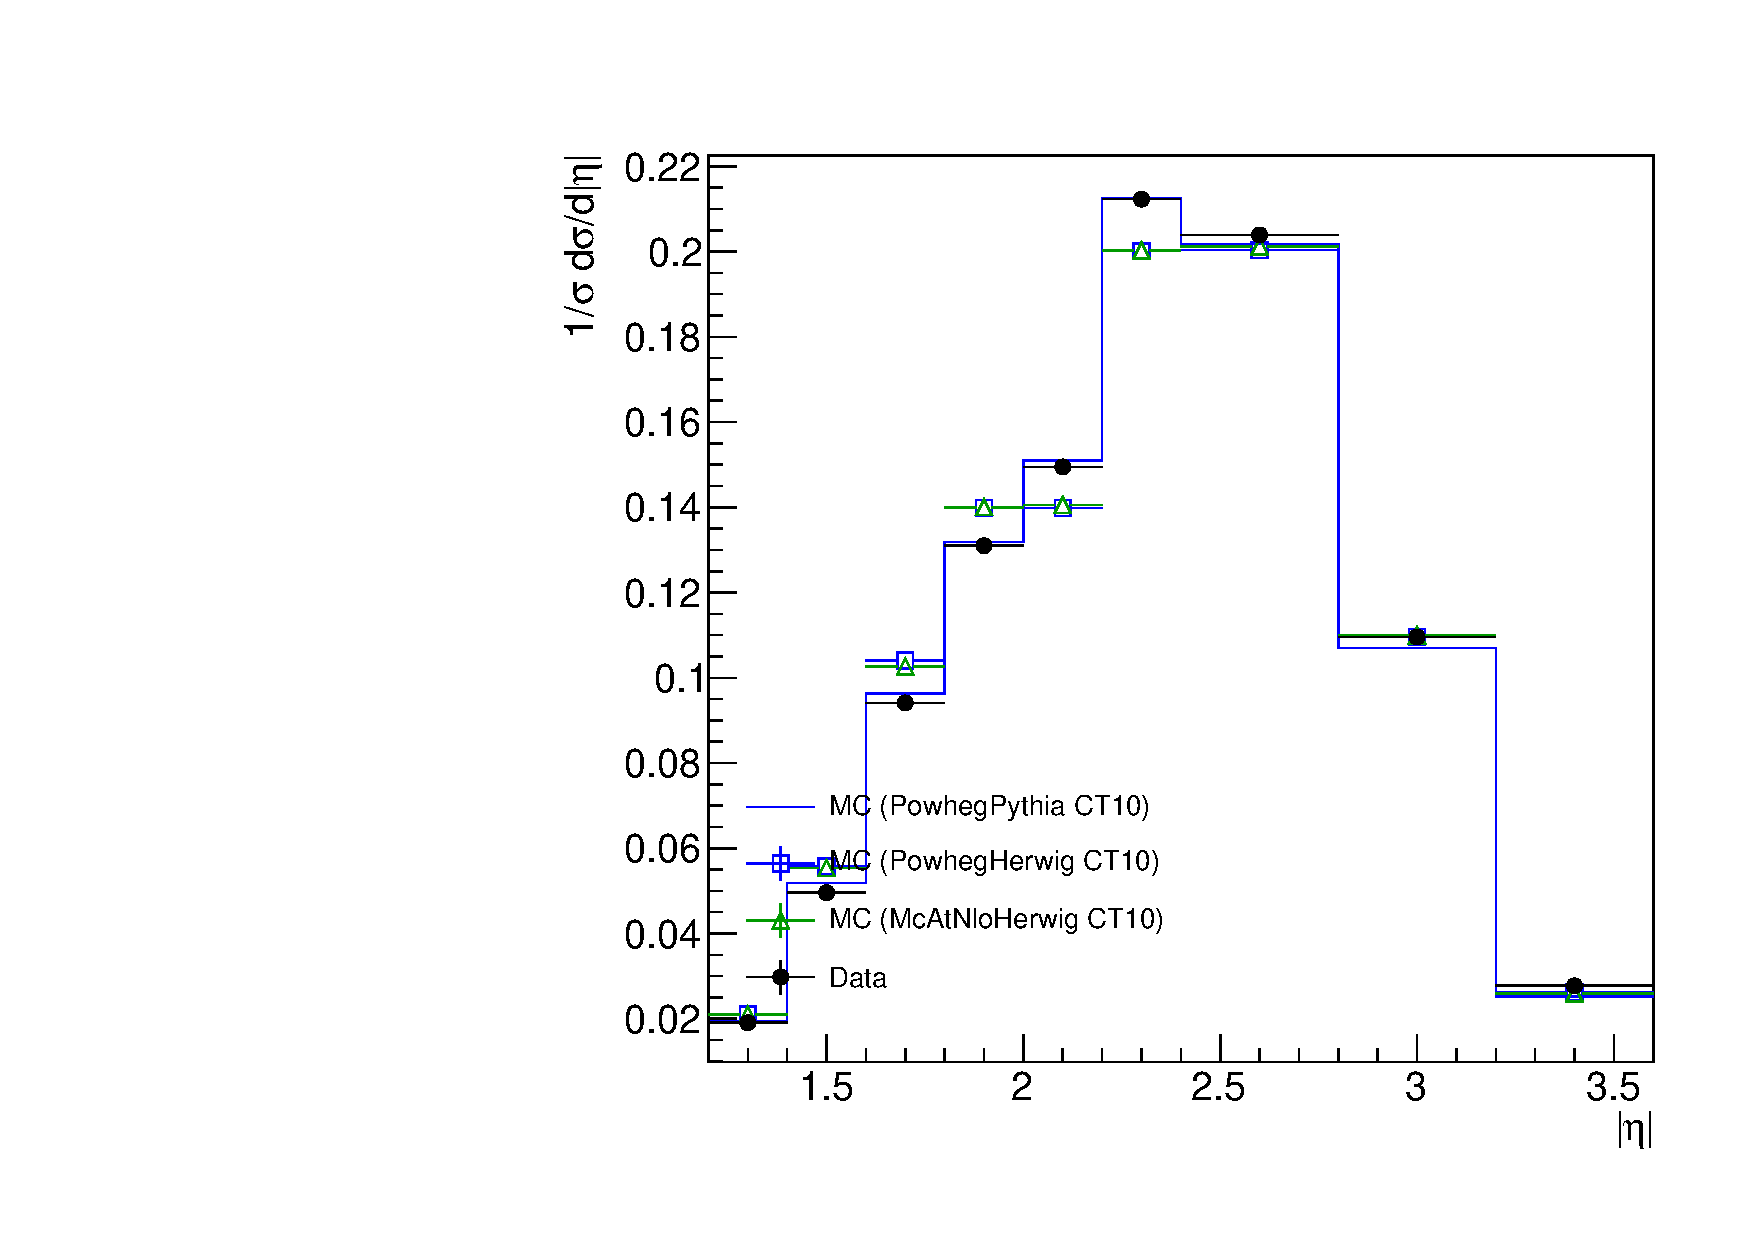
\includegraphics[width=0.45\textwidth]{figures/ZeeCF_Mass_66_116_FiduCS.pdf}
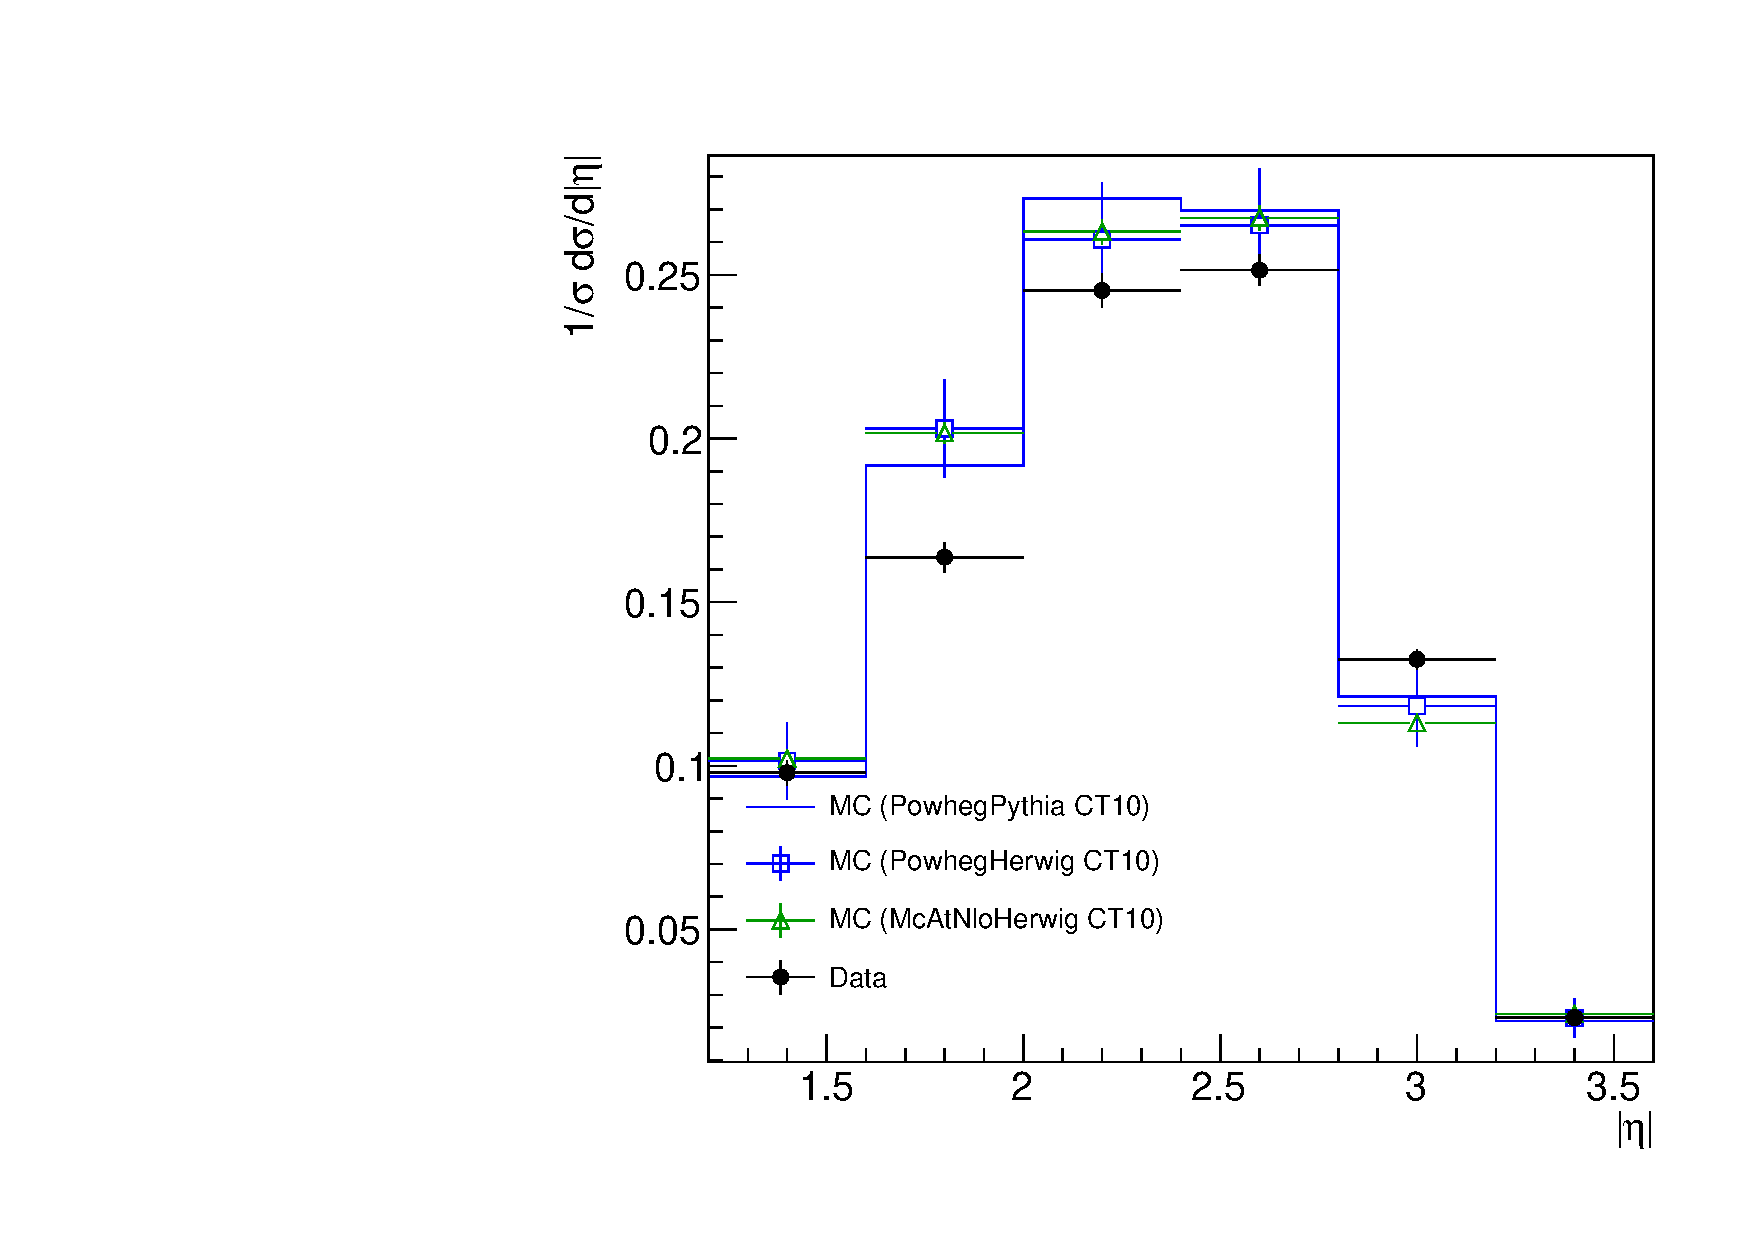
\includegraphics[width=0.45\textwidth]{figures/ZeeCF_Mass_116_150_FiduCS.pdf}
\caption{Normalised \Zee\ CF differential cross-section, as a function of absolute boson rapidity for peak mass (left) and high mass (right) regions.}
\label{fig:res_zee_fid_norm}}
\end{figure}

The same results in tabular form can be seen in Tabs.~\ref{tab:Zee_NBC_peak} and~\ref{tab:Zee_NBC_high}, where $N$ is the number of events in the bin, $B$ is the estimated number of the background events included in $N$, and $C$ is the genuinely experimental fiducial extrapolation factor, which represents the fraction of all the $Z$ boson that $N$ amounts to.

\begin{table}
\centering
\begin{tabular}{lccc}
\hline
    &   $N$   & $B \pm \delta B$  &  $C \pm \delta C$ \\
\hline
$1.20 < |\eta| <1.40$          & 4178       & 193.7      $\pm$ 19.7 & 0.381      $\pm$ 0.014 \\
$1.40 < |\eta| <1.60$          & 12404      & 517.7      $\pm$ 47.4 & 0.436      $\pm$ 0.013 \\
$1.60 < |\eta| <1.80$          & 24210      & 812.1      $\pm$ 72.7 & 0.453      $\pm$ 0.012 \\
$1.80 < |\eta| <2.00$          & 33978      & 1021.2     $\pm$ 110.9 & 0.459      $\pm$ 0.014 \\
$2.00 < |\eta| <2.20$          & 38023      & 1141.2     $\pm$ 123.9 & 0.449      $\pm$ 0.015 \\
$2.20 < |\eta| <2.40$          & 51372      & 1454.4     $\pm$ 77.6 & 0.429      $\pm$ 0.011 \\
$2.40 < |\eta| <2.80$          & 101004     & 2613.2     $\pm$ 267.5 & 0.440      $\pm$ 0.015 \\
$2.80 < |\eta| <3.20$          & 47304      & 1104.4     $\pm$ 52.3 & 0.384      $\pm$ 0.021 \\
$3.20 < |\eta| <3.60$          & 8453       & 126.6      $\pm$ 29.5 & 0.276      $\pm$ 0.020 \\
\hline
\end{tabular}
\caption{Main components of the differential \Zee\ CF cross-section for peak mass region.}
\label{tab:Zee_NBC_peak}
\end{table}

\begin{table}
\centering
\begin{tabular}{lccc}
\hline
    &   $N$   & $B \pm \delta B$  &  $C \pm \delta C$ \\
\hline
$1.20 < |\eta| <1.60$          & 1136       & 592.4      $\pm$ 54.8 & 0.552      $\pm$ 0.024 \\
$1.60 < |\eta| <2.00$          & 1676       & 754.6      $\pm$ 79.2 & 0.565      $\pm$ 0.035 \\
$2.00 < |\eta| <2.40$          & 2006       & 737.4      $\pm$ 80.2 & 0.531      $\pm$ 0.067 \\
$2.40 < |\eta| <2.80$          & 1754       & 506.2      $\pm$ 48.6 & 0.515      $\pm$ 0.107 \\
$2.80 < |\eta| <3.20$          & 659        & 120.7      $\pm$ 12.8 & 0.439      $\pm$ 0.068 \\
$3.20 < |\eta| <3.60$          & 84         & 15.2       $\pm$ 8.3 & 0.348      $\pm$ 0.031 \\
\hline
\end{tabular}
\caption{Main components of the differential \Zee\ CF cross-section for high mass region.}
\label{tab:Zee_NBC_high}
\end{table}

In Tabs.~\ref{tab:Zee_peak} and~\ref{tab:Zee_high} the results of the cross-section as measured in the experimental fiducial volume can be found along with statistical, systematical and luminosity uncertainties.

\begin{table}
\centering
\begin{tabular}{lc}
\hline
$1.20 < |\eta| <1.40$          & 5.715 $\pm$ 0.101 (stat) $\pm$ 0.207 (syst) $\pm$ 0.103 (lum) [pb]  \\
$1.40 < |\eta| <1.60$          & 14.864 $\pm$ 0.151 (stat) $\pm$ 0.465 (syst) $\pm$ 0.268 (lum) [pb]  \\
$1.60 < |\eta| <1.80$          & 28.200 $\pm$ 0.206 (stat) $\pm$ 0.792 (syst) $\pm$ 0.508 (lum) [pb]  \\
$1.80 < |\eta| <2.00$          & 39.245 $\pm$ 0.233 (stat) $\pm$ 1.214 (syst) $\pm$ 0.706 (lum) [pb]  \\
$2.00 < |\eta| <2.20$          & 44.786 $\pm$ 0.260 (stat) $\pm$ 1.534 (syst) $\pm$ 0.806 (lum) [pb]  \\
$2.20 < |\eta| <2.40$          & 63.598 $\pm$ 0.317 (stat) $\pm$ 1.717 (syst) $\pm$ 1.145 (lum) [pb]  \\
$2.40 < |\eta| <2.80$          & 61.087 $\pm$ 0.207 (stat) $\pm$ 2.126 (syst) $\pm$ 1.100 (lum) [pb]  \\
$2.80 < |\eta| <3.20$          & 32.826 $\pm$ 0.162 (stat) $\pm$ 1.811 (syst) $\pm$ 0.591 (lum) [pb]  \\
$3.20 < |\eta| <3.60$          & 8.313 $\pm$ 0.102 (stat) $\pm$ 0.614 (syst) $\pm$ 0.150 (lum) [pb]  \\
\hline
\end{tabular}
\caption{Differential \Zee\ CF cross-section for the peak mass region, measured in the experimental fiducial volume together with uncertainties.}
\label{tab:Zee_peak}
\end{table}

\begin{table}
\centering
\begin{tabular}{lc}
\hline
$1.20 < |\eta| <1.60$          & 0.271 $\pm$ 0.018 (stat) $\pm$ 0.030 (syst) $\pm$ 0.005 (lum) [pb]  \\
$1.60 < |\eta| <2.00$          & 0.454 $\pm$ 0.023 (stat) $\pm$ 0.047 (syst) $\pm$ 0.008 (lum) [pb]  \\
$2.00 < |\eta| <2.40$          & 0.680 $\pm$ 0.027 (stat) $\pm$ 0.095 (syst) $\pm$ 0.012 (lum) [pb]  \\
$2.40 < |\eta| <2.80$          & 0.697 $\pm$ 0.027 (stat) $\pm$ 0.147 (syst) $\pm$ 0.013 (lum) [pb]  \\
$2.80 < |\eta| <3.20$          & 0.367 $\pm$ 0.019 (stat) $\pm$ 0.057 (syst) $\pm$ 0.007 (lum) [pb]  \\
$3.20 < |\eta| <3.60$          & 0.064 $\pm$ 0.009 (stat) $\pm$ 0.009 (syst) $\pm$ 0.001 (lum) [pb]  \\
\hline
\end{tabular}
\caption{Differential \Zee\ CF cross-section for the high mass region, measured in the experimental fiducial volume together with uncertainties.}
\label{tab:Zee_high}
\end{table}

And finally in Tabs~\ref{tab:Zee_NBC} and~\ref{tab:Zee} the results for integrated cross-sections can be found.

\begin{table}
\centering
\begin{tabular}{lccc}
\hline
    &   $N$   & $B \pm \delta B$  &  $C \pm \delta C$ \\
\hline
$\hfill 66.00 < m_{ee} <116.00$       & 321575     & 9174.1     $\pm$ 462.1 & 0.425      $\pm$ 0.010 \\
$116.00 < m_{ee} <150.00$      & 7740       & 2732.8     $\pm$ 261.8 & 0.520      $\pm$ 0.018 \\
\hline
\end{tabular}
\caption{Main components of the integrated \Zee\ CF cross-section.}
\label{tab:Zee_NBC}
\end{table}

\begin{table}
\centering
\begin{tabular}{lc}
\hline
$\hfill 66.00 < m_{ee} <116.00$       & 3.204 $\pm$ 0.006 (stat) $\pm$ 0.073 (syst) $\pm$ 0.058 (lum) [pb]  \\
$116.00 < m_{ee} <150.00$      & 0.063 $\pm$ 0.001 (stat) $\pm$ 0.004 (syst) $\pm$ 0.001 (lum) [pb]  \\
\hline
\end{tabular}
\caption{Integrated \Zee\ CF cross-section, measured in the experimental fiducial volume together with uncertainties.}
\label{tab:Zee}
\end{table}

The comparison with the theoretical predictions was done for the combined \Zll\ results. Since the combination itself was outside of the scope of this thesis, it won't be described here. It is important to note, that \Zee central-forward data contributed only to the $|y| > 1.2$ part of the combined cross-section, and the last three bins $|y| > 2.4$ of it can be seen as purely \Zee\ central-forward. The combined cross-section itself can be seen in Fig.~\ref{fig:Zll}, while the comparison with the different theoretical predictions can be seen in Fig.~\ref{fig:Zll_theory}.

\begin{figure}
\center{
  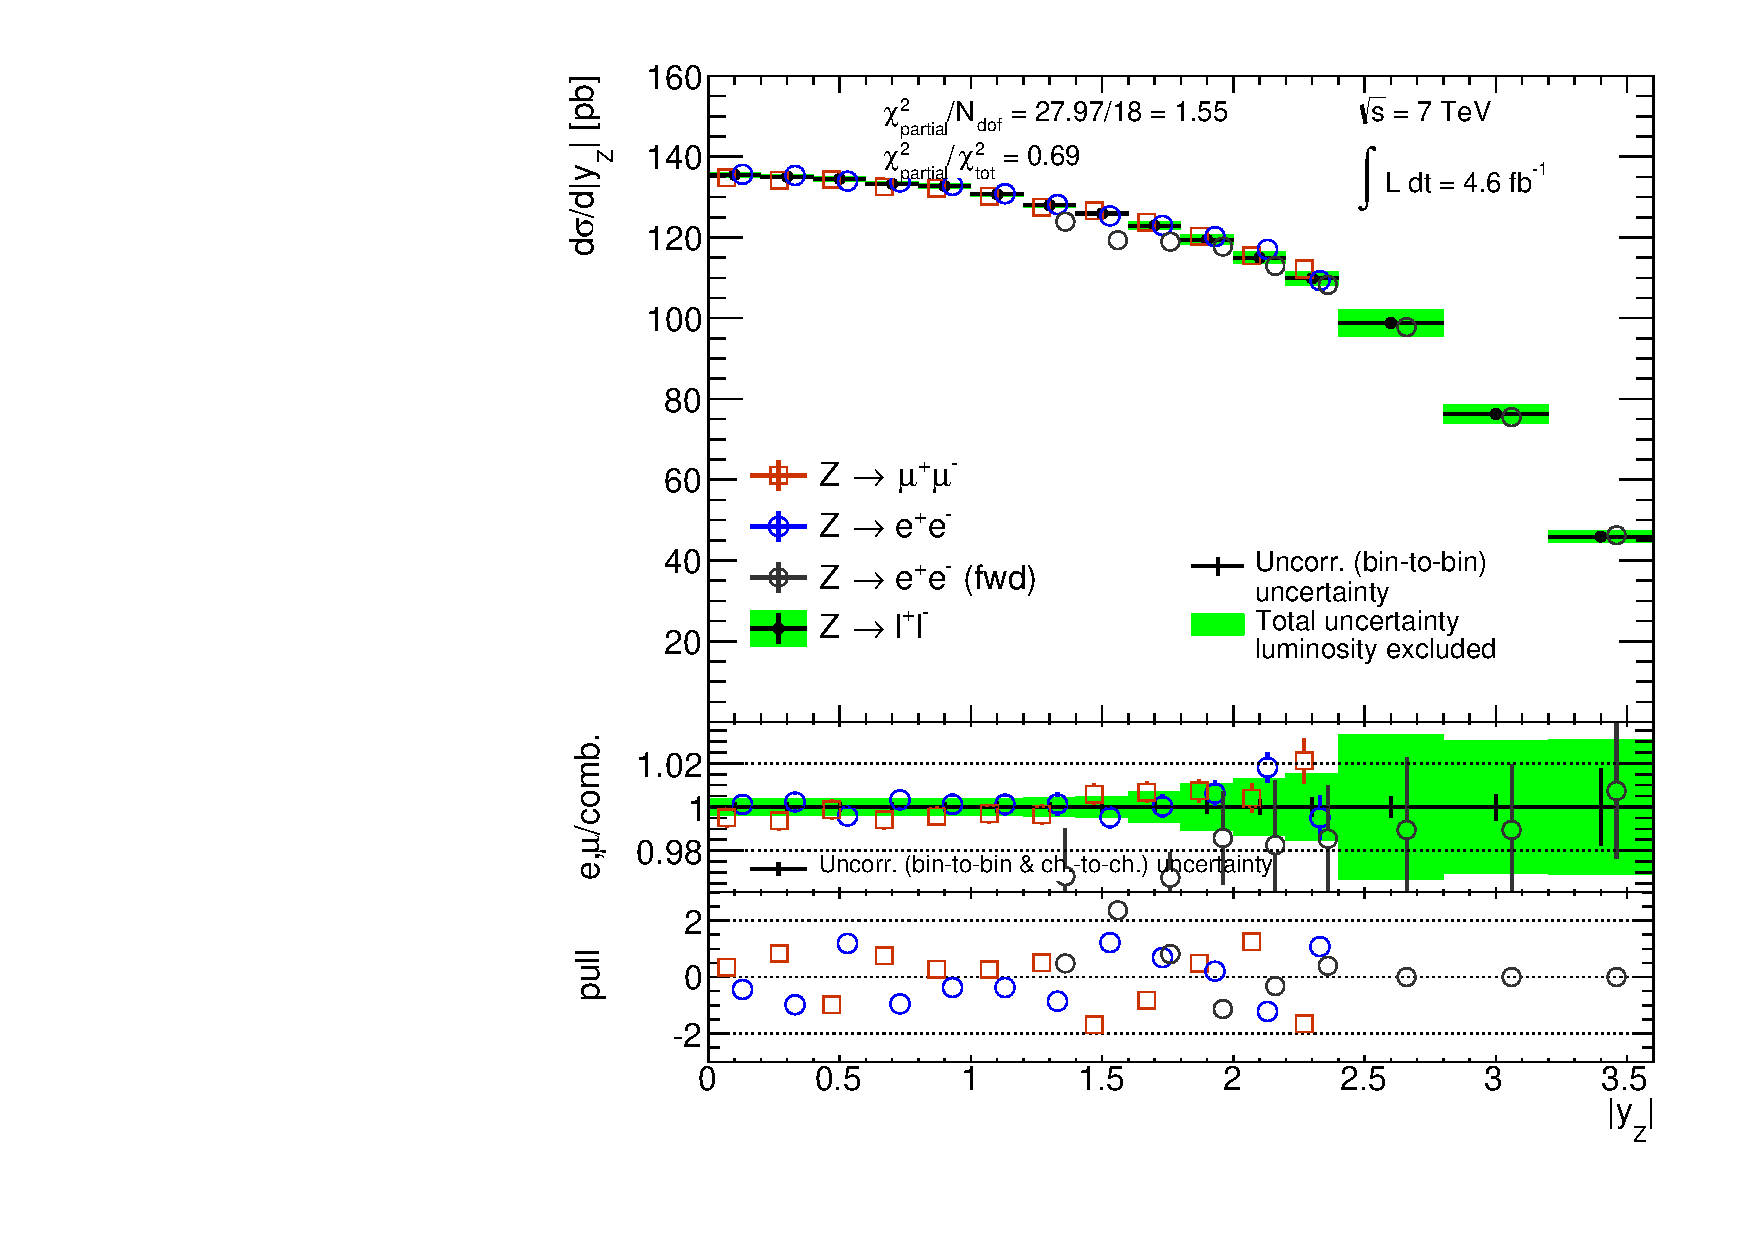
\includegraphics[width=0.45\textwidth]{figures/Z_66_116_combined.pdf}
  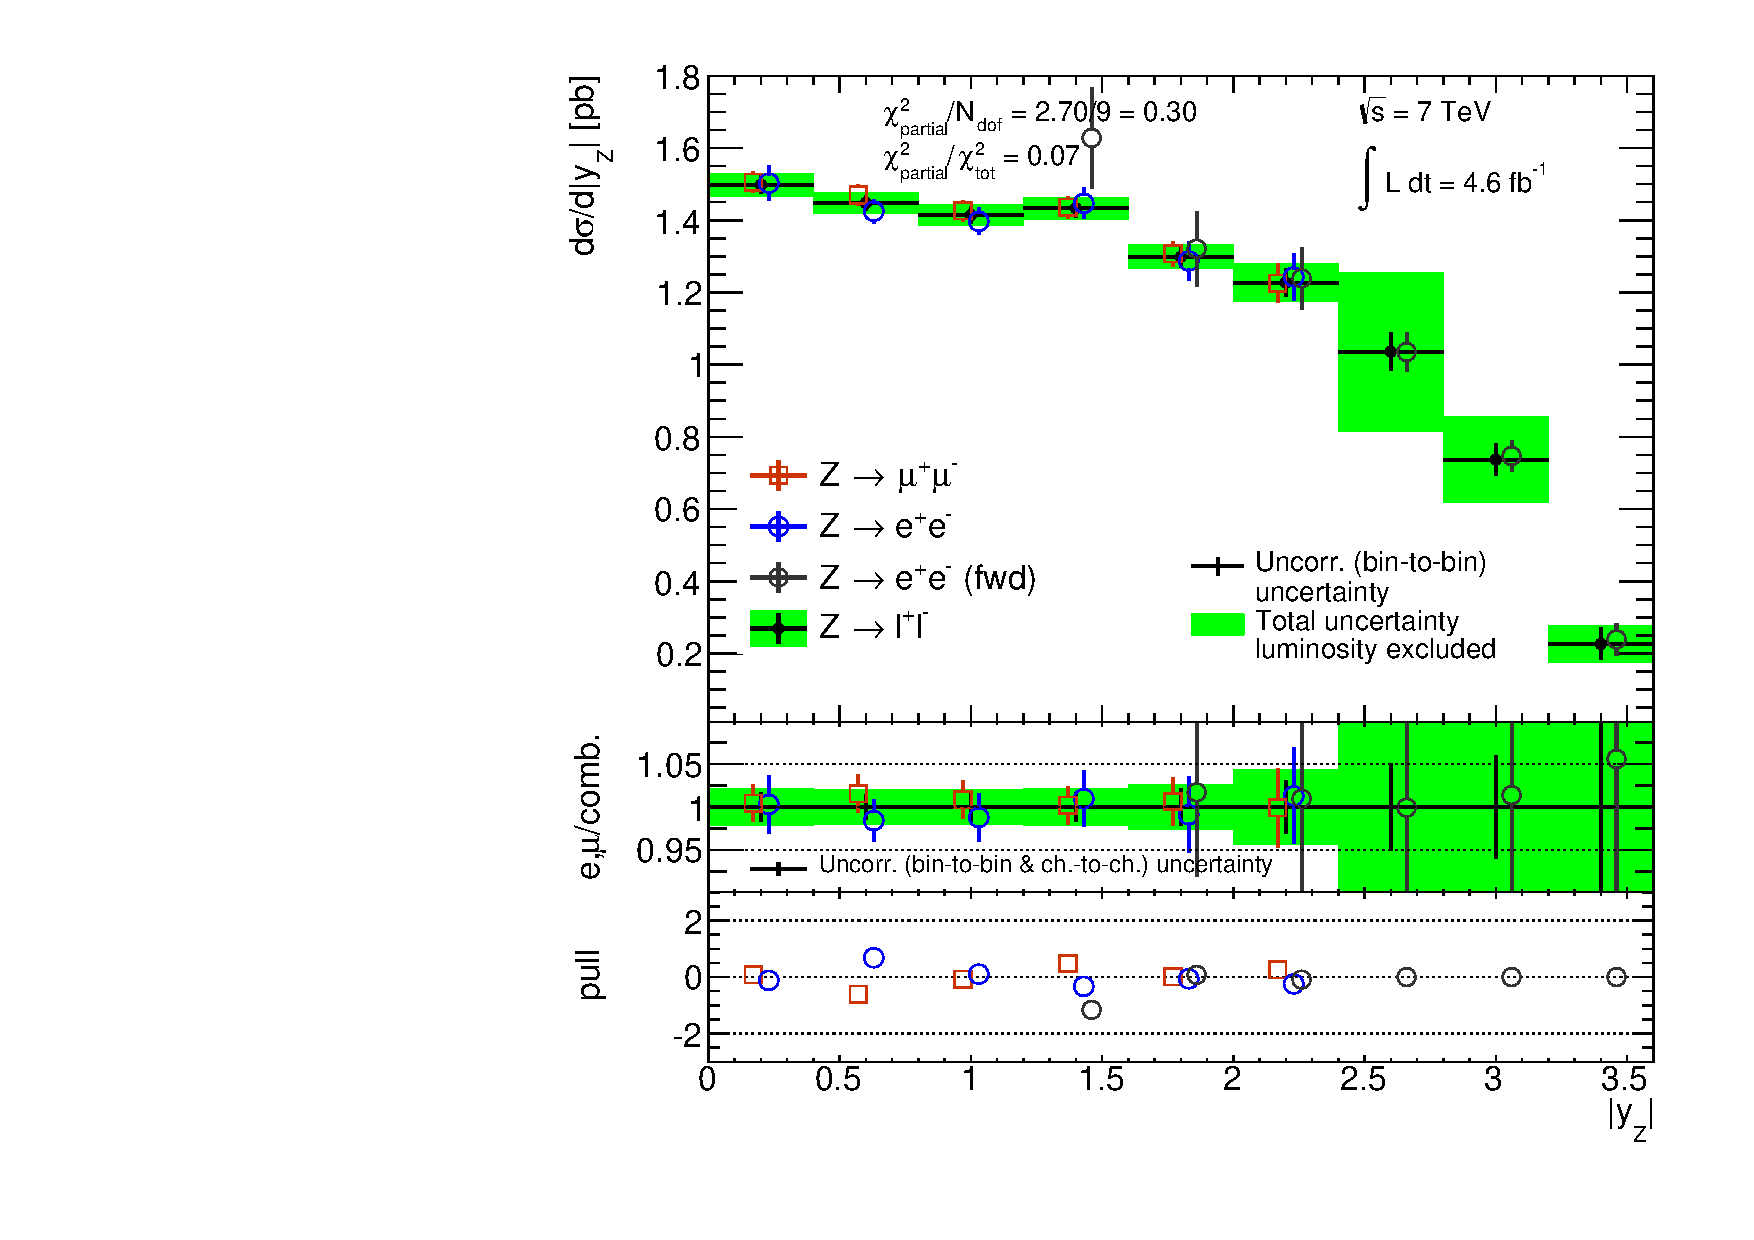
\includegraphics[width=0.45\textwidth]{figures/Z_116_150_combined.pdf}
  \caption{Combined \Zll\ cross-section for peak mass (left) and high mass (right) regions together with uncertainties. The ratio and the pull values are also shown for each source.}
\label{fig:Zll}}
\end{figure}

\begin{figure}
\center{
  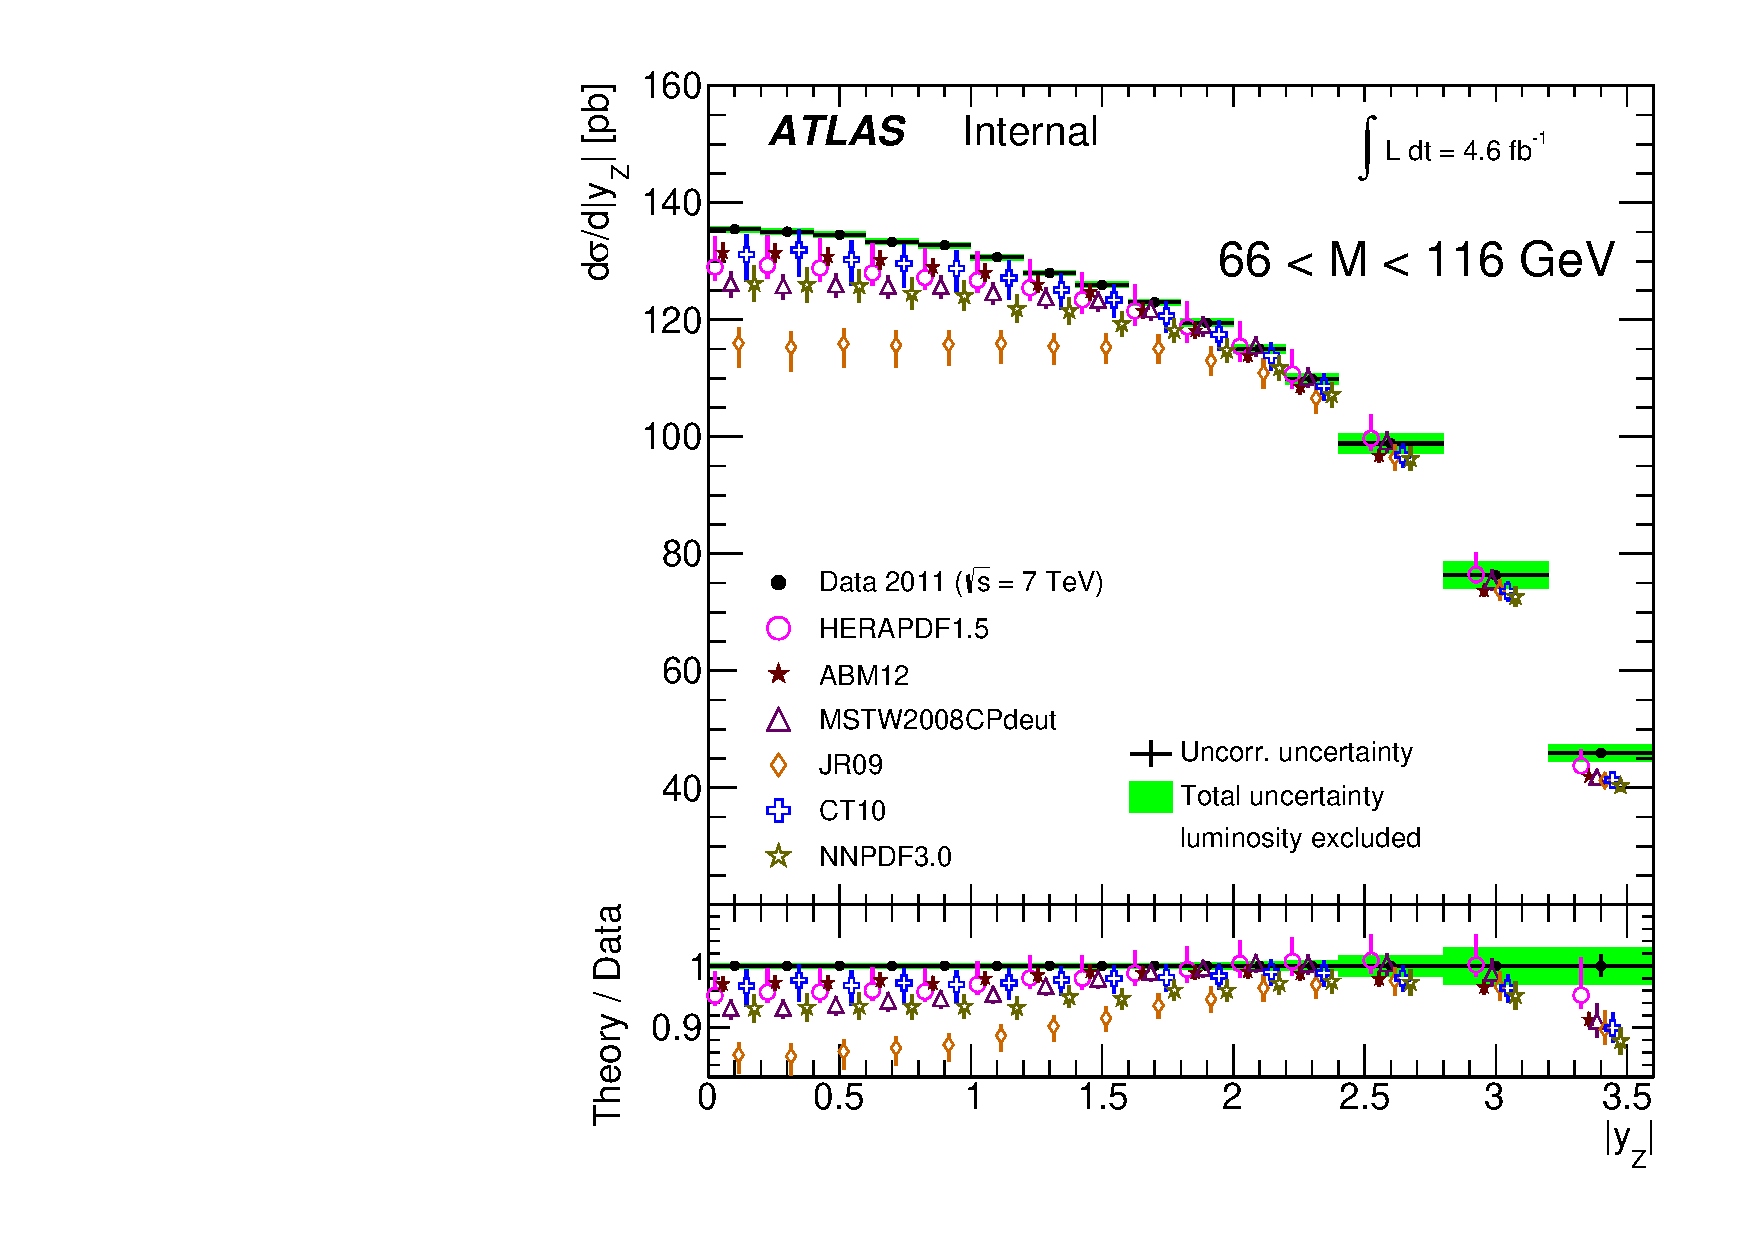
\includegraphics[width=0.45\textwidth]{figures/Z_66_116_NNLO_combined.pdf}
  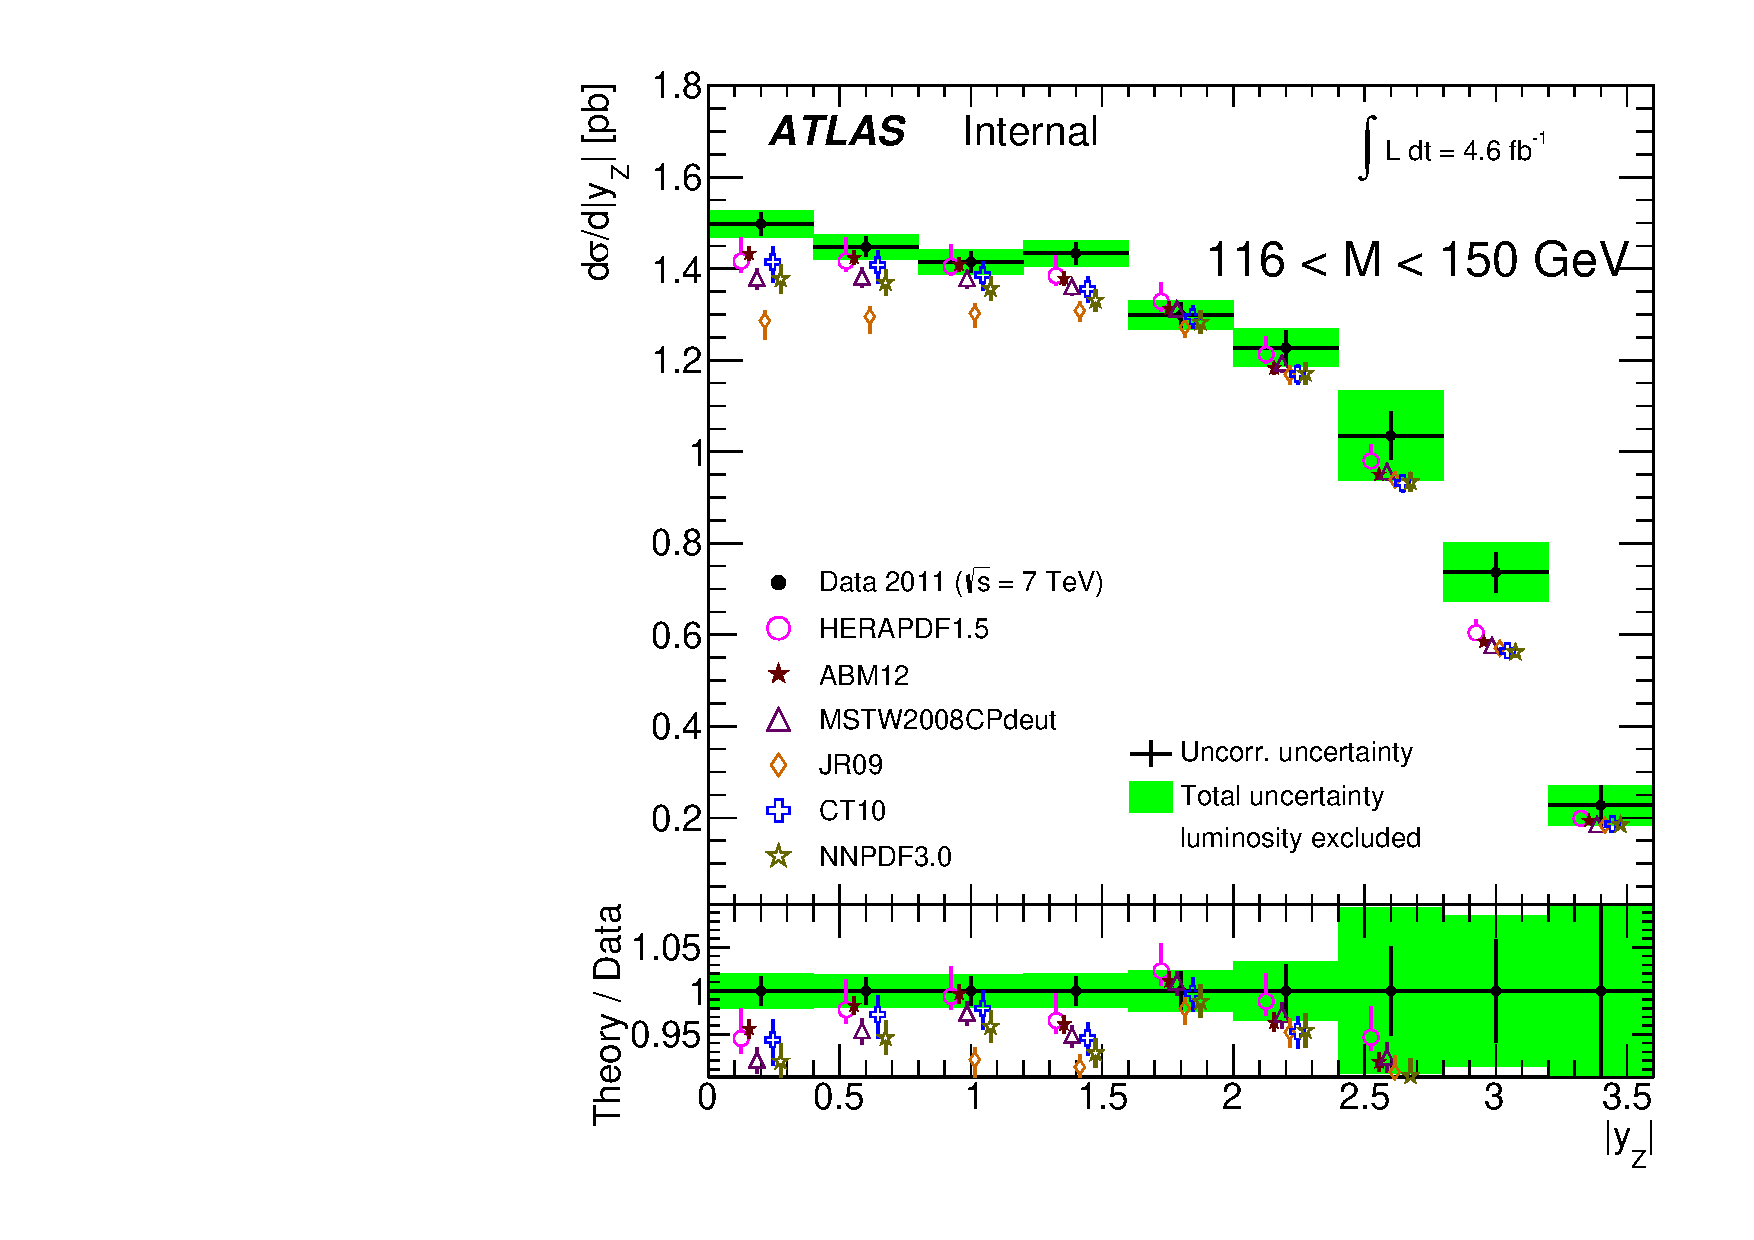
\includegraphics[width=0.45\textwidth]{figures/Z_116_150_NNLO_combined.pdf}
  \caption{Comparison of the combined \Zll\ cross-section with NNLO predictions using varios PDF sets for peak mass (left) and high mass (right) regions together with uncertainties. The ratios are also shown.}
\label{fig:Zll_theory}}
\end{figure}
